% =====================================================================
%  Documento Final del Proyecto
%  Sistema Web de Gestion de Cursos, Eventos e Inscripciones Academicas
%  Equipo: Gallegos, Gallardo, Diaz, Nava  -  UAZ, Junio 2026
%  Compilar con:  pdflatex documento_final.tex  (dos pasadas)
% =====================================================================
\documentclass[11pt,letterpaper]{article}

\usepackage[utf8]{inputenc}
\usepackage[T1]{fontenc}
\usepackage[spanish,es-tabla]{babel}
\usepackage{lmodern}
\usepackage[margin=2.5cm]{geometry}
\usepackage{graphicx}
\usepackage{xcolor}
\usepackage{enumitem}
\usepackage{tabularx}
\usepackage{longtable}
\usepackage{array}
\usepackage{booktabs}
\usepackage{colortbl}
\usepackage{titlesec}
\usepackage{fancyhdr}
\usepackage{hyperref}
\usepackage{tcolorbox}
\usepackage{caption}
\usepackage{float}    
\usepackage{microtype}
\usepackage{subcaption}

% --- colores ---------------------------------------------------------
\definecolor{azulUAZ}{HTML}{1F4E79}
\definecolor{azulSec}{HTML}{2E74B5}
\definecolor{grisCap}{HTML}{F2F2F2}
\definecolor{grisTxt}{HTML}{595959}
\definecolor{grisAlt}{HTML}{F2F2F2}

% --- titulos ---------------------------------------------------------
\titleformat{\section}{\Large\bfseries\color{azulUAZ}}{\thesection.}{0.6em}{}
\titleformat{\subsection}{\large\bfseries\color{azulSec}}{\thesubsection}{0.6em}{}
\titleformat{\subsubsection}{\normalsize\bfseries\color{azulSec}}{\thesubsubsection}{0.6em}{}

% --- hipervinculos ---------------------------------------------------
\hypersetup{
	colorlinks=true,
	linkcolor=azulSec,
	urlcolor=azulSec,
	citecolor=azulSec,
	pdftitle={Documento Final - Sistema de Gestion de Cursos},
	pdfauthor={Equipo SCEA - UAZ}
}

% --- encabezado/pie --------------------------------------------------
\pagestyle{fancy}
\fancyhf{}
\fancyfoot[C]{\small\color{grisTxt} Pagina \thepage{} de \pageref{LastPage}}
\renewcommand{\headrulewidth}{0pt}
\usepackage{lastpage}

% --- figura con imagen real ------------------------------------------
\newcommand{\figura}[3][1.0]{%
	\begin{figure}[H]
		\centering
		\includegraphics[width=#1\linewidth]{#2}
		\caption{#3}
	\end{figure}
	\vspace{0.4em}
}
% --- marcador de captura de pantalla (sin imagen disponible) ---------
\newcommand{\captura}[1]{%
	\begin{center}
		\begin{tcolorbox}[colback=grisCap,colframe=grisCap,boxrule=0pt,
			arc=2pt,left=8pt,right=8pt,top=4pt,bottom=4pt,width=\linewidth]
			\centering\itshape\color{grisTxt}\small [Captura de pantalla: #1]
		\end{tcolorbox}
	\end{center}%
	\vspace{-0.4em}
	\begin{center}\small\itshape\color{grisTxt} Figura. #1\end{center}
	\vspace{0.6em}
}

% --- formato de tablas -----------------------------------------------
\renewcommand{\arraystretch}{1.25}
\arrayrulecolor{black!30}
\newcommand{\headrowcolor}{\rowcolor{azulUAZ}}
\newcommand{\headcell}[1]{\textcolor{white}{\textbf{#1}}}

% =====================================================================
\begin{document}
	
	% ======================== PORTADA =====================================
	\thispagestyle{empty}
	\thispagestyle{empty}
	\begin{center}
		\vspace*{0.1cm}
		
\includegraphics[width=0.85\linewidth]{img/cabeceralogo_elec.png}\\[1cm]
		
		% Aumentamos tamaño a \huge y el espacio entre renglones a [0.6em]
		{\huge\bfseries UNIVERSIDAD AUT\'ONOMA DE \\[0.5em]
			ZACATECAS}\\[0.6em]
		{\Large Unidad Acad\'emica de Ingenier\'ia El\'ectrica}\\[0.4em]
		{\Large\itshape Programa de Ingenier\'ia de Software}
		
		% Espacio fijo en lugar de \vfill para que no se disperse tanto
		\vspace{1.5cm} 
		
		% El título se queda en \Huge como pediste, pero ampliamos su interlineado interno a [0.8em]
		{\Huge\bfseries Sistema Web de Gesti\'on\\[0.3em] de Cursos, Eventos\\[0.3em] e Inscripciones Acad\'emicas}\\[1.2cm]
		
		% Subtítulo aumentado a \LARGE
		{\LARGE\itshape Documento Final de Proyecto}
		
		\vspace{1.5cm}
		
		% Sección de integrantes con letra \large e interlineado de [0.5em] entre nombres
		{\Large\bfseries Integrantes del equipo:}\\[0.8em]
		{\large Mar\'ia de los \'Angeles Gallegos Ba\~nuelos}\\[0.5em]
		{\large Camila Alejandra Gallardo Torres}\\[0.5em]
		{\large Blanca Esthela D\'iaz Hern\'andez}\\[0.5em]
		{\large Jos\'e Efra\'in Nava Favela}
		
		\vspace{1.5cm}
		
		% Datos de la materia en \large y con más interlineado interno
		{\large
			Materia: Pruebas y mantenimiento de software\\[0.5em]
			Docente: MSc.\ Alejandro Isais Torres\\[0.5em]
			Fecha de entrega: Junio 2026}
	\end{center}	
	\newpage
	
	% ======================== 1. INTRODUCCION =============================
	\section{Introducci\'on}
	El presente documento describe el desarrollo del \textbf{Sistema Web de Gesti\'on de Cursos, Eventos e Inscripciones Acad\'emicas}, una aplicaci\'on web desarrollada como proyecto final de la materia de Programaci\'on Delphi utilizando Django~4.2 y Django REST Framework.
	
	El proyecto surge de la necesidad de mejorar la administraci\'on de cursos y eventos acad\'emicos dentro de una instituci\'on educativa, ya que los procesos realizados de forma manual suelen generar problemas relacionados con la organizaci\'on, consulta y control de la informaci\'on. Para atender esta problem\'atica se desarroll\'o una plataforma que permite centralizar la gesti\'on de usuarios, cursos, inscripciones y evidencias digitales, incorporando mecanismos de validaci\'on y control de acceso que contribuyen a mantener la integridad de los datos.
	
	Durante el desarrollo se aplicaron conceptos relacionados con modelado de datos, dise\~no de interfaces, autenticaci\'on de usuarios, control de permisos, validaci\'on de informaci\'on y exposici\'on de servicios mediante una API REST. Esto permiti\'o construir una soluci\'on funcional capaz de responder a los requerimientos planteados para el proyecto.
	
	En las siguientes secciones se presenta el planteamiento del problema, los objetivos, el alcance del sistema, los requerimientos funcionales y no funcionales, las reglas de negocio, el modelo de datos, las vistas implementadas, la API REST, las pruebas realizadas y las conclusiones obtenidas durante el desarrollo.
		
	% ======================== 2. PLANTEAMIENTO ============================
	\section{Planteamiento del problema}
	Una instituci\'on educativa que imparte cursos y eventos de formaci\'on acad\'emica realiza actualmente sus procesos de inscripci\'on de manera manual, utilizando hojas de c\'alculo y registros en papel. Esta situaci\'on genera los siguientes problemas:
	\begin{itemize}[leftmargin=*]
		\item P\'erdida de informaci\'on: los registros f\'isicos se deterioran, se extrav\'ian o se duplican.
		\item Duplicidad de inscripciones: un alumno puede registrarse varias veces al mismo curso sin que exista un mecanismo autom\'atico de validaci\'on.
		\item Dificultad de consulta: no hay una forma r\'apida de saber cu\'antos alumnos est\'an inscritos en un curso, qui\'en los imparte o cu\'al es el estado actual de cada evento.
		\item Falta de trazabilidad: no se cuenta con evidencia digital que respalde la participaci\'on de los alumnos.
		\item Ausencia de control de cupo: los cursos pueden sobrepasar su capacidad m\'axima sin que el sistema lo impida.
	\end{itemize}
	La soluci\'on propuesta es una aplicaci\'on web centralizada que automatice el registro, la inscripci\'on y la consulta de informaci\'on acad\'emica, garantizando la integridad de los datos mediante validaciones en el servidor y reglas de negocio claras y reproducibles.
	
	% ======================== 3. OBJETIVO GENERAL =========================
	\section{Objetivo general}
	Desarrollar una aplicaci\'on web para la gesti\'on de cursos, eventos e inscripciones acad\'emicas mediante el uso de Django~4.2 y Django REST Framework, integrando mecanismos de autenticaci\'on, control de acceso por roles, validaci\'on de datos, manejo de archivos y servicios REST, con la finalidad de centralizar la informaci\'on y optimizar los procesos administrativos de una instituci\'on educativa.
	
	% ======================== 4. OBJETIVOS ESPECIFICOS ====================
	\section{Objetivos espec\'ificos}
	\begin{enumerate}[leftmargin=*]
		\item Implementar un sistema de autenticaci\'on con tres roles de usuario (Administrador, Instructor y Alumno), utilizando el modelo de a\\
		utenticaci\'on nativo de Django extendido con la entidad \texttt{PerfilUsuario}.
		\item Crear el m\'odulo de gesti\'on de cursos con operaciones CRUD completas restringidas al rol de administrador, incluyendo carga de im\'agenes asociadas.
		\item Desarrollar el m\'odulo de inscripciones con validaciones de cupo m\'aximo, estado del curso e inscripciones duplicadas, permitiendo adem\'as la carga de evidencias o comprobantes por parte del alumno.
		\item Implementar vistas basadas en clases (\texttt{ListView}, \texttt{DetailView}, \texttt{CreateView}, \texttt{UpdateView}, \texttt{DeleteView}) en al menos los m\'odulos de cursos, alumnos, instructores e inscripciones administrativas.
		\item Dise\~nar formularios personalizados con \texttt{ModelForms} que incluyan validaciones propias en campos como nombre, correo, cupo m\'aximo, fechas y archivos.
		\item Exponer una API REST con Django REST Framework que permita realizar operaciones CRUD sobre cursos, alumnos, inscripciones e instructores, mediante \texttt{ViewSets} y \texttt{serializers} con permisos por rol.
		\item Proveer una interfaz web responsiva construida con Bootstrap~5.3 que permita a los usuarios localizar cualquier funcionalidad en menos de 20 segundos.
	\end{enumerate}
	
	% ======================== 5. ALCANCE ==================================
	\section{Alcance del sistema}
	El sistema abarca los siguientes m\'odulos y funcionalidades dentro de un entorno de ejecuci\'on local:
	\begin{itemize}[leftmargin=*]
		\item \textbf{Gesti\'on de usuarios:} registro p\'ublico exclusivo para alumnos (decisi\'on de seguridad: no se permite elegir rol en el registro), inicio y cierre de sesi\'on, vista de perfil. Los roles instructor y administrador los asigna manualmente el administrador.
		\item \textbf{Gesti\'on de alumnos e instructores:} CRUD completo restringido a administradores. Al crear un instructor, el admin registra en un solo paso la ficha acad\'emica y la cuenta de acceso (\texttt{User} + \texttt{PerfilUsuario} + \texttt{Instructor}) dentro de una transacci\'on at\'omica. Fotograf\'ia opcional solo en alumnos.
		\item \textbf{Gesti\'on de cursos:} CRUD con imagen opcional, estado (activo, cerrado, cancelado), cupo m\'aximo e instructor asignado; restringido a administradores. Vista web \emph{Mis cursos} para instructores autenticados.
		\item \textbf{Inscripciones:} inscripci\'on del alumno, vista \emph{Mis Inscripciones} y carga de evidencias para alumnos; CRUD web de inscripciones para administradores en \texttt{/inscripciones/gestion/}.
		\item \textbf{Evidencias:} carga de archivos PDF, im\'agenes o documentos Word como comprobante de inscripci\'on.
		\item \textbf{B\'usqueda y filtrado:} por nombre de curso, instructor y estado.
		\item \textbf{API REST:} endpoints para cursos, alumnos, inscripciones e instructores con autenticaci\'on por sesi\'on y permisos por rol.
		\item \textbf{Navegaci\'on por rol} en la barra principal: \emph{Mis Inscripciones} solo para alumnos; \emph{Mis Cursos} solo para instructores; men\'u \emph{Administrar} solo para administradores.
	\end{itemize}
	Queda fuera del alcance de este proyecto: el despliegue en servidores de producci\'on, la integraci\'on con sistemas de pago, la generaci\'on autom\'atica de certificados y el env\'io de correos electr\'onicos.
	
	% ======================== 6. USUARIOS =================================
	\section{Usuarios del sistema}
	El sistema define tres roles diferenciados con capacidades espec\'ificas:
	
	\begin{center}\small
		\begin{tabularx}{\linewidth}{|>{\bfseries}l|X|X|}
			\hline
			\headrowcolor \headcell{Rol} & \headcell{Descripci\'on} & \headcell{Capacidades principales} \\ \hline
			Administrador & Usuario con acceso total al sistema. & CRUD web de cursos, alumnos, instructores e inscripciones. Acceso al men\'u Administrar y al panel \texttt{/admin/}. No se auto-inscribe a cursos; usa la gesti\'on administrativa de inscripciones. \\ \hline
			\rowcolor{grisAlt}
			Instructor & Docente que imparte uno o m\'as cursos. & Vista \emph{Mis cursos} (\texttt{/cursos/mis-cursos/}), detalle del curso y consulta de alumnos inscritos en los cursos que imparte. No se auto-inscribe a cursos. \\ \hline
			Alumno & Estudiante que se inscribe a cursos. & Registro p\'ublico, vista \emph{Mis Inscripciones}, inscripci\'on en l\'inea desde el detalle del curso y carga de evidencias digitales por inscripci\'on. \\ \hline
		\end{tabularx}
	\end{center}
		
	\vspace{1cm}		
	\begin{figure}[H]
		\centering
		% 1. Vista Administrador
		\begin{subfigure}[b]{0.31\linewidth}
			\centering
			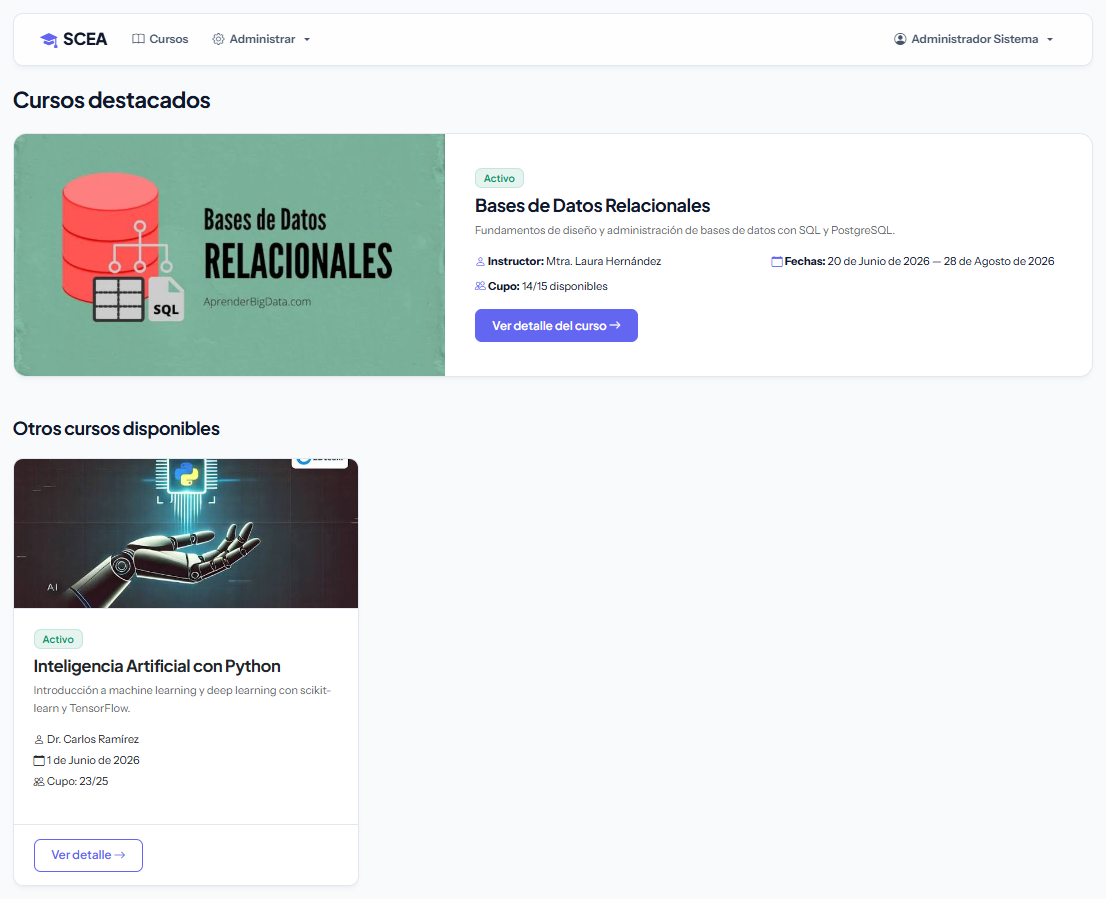
\includegraphics[width=\linewidth]{img/capturas_app/pagina_administrador.png}
			\caption{Vista Administrador}
		\end{subfigure}%
		\hfill
		% 2. Vista Instructor
		\begin{subfigure}[b]{0.31\linewidth}
			\centering
			
\includegraphics[width=\linewidth]{img/capturas_app/pagina_instructor.png}
			\caption{Vista Instructor}
		\end{subfigure}%
		\hfill
		% 3. Vista Alumno
		\begin{subfigure}[b]{0.31\linewidth}
			\centering
			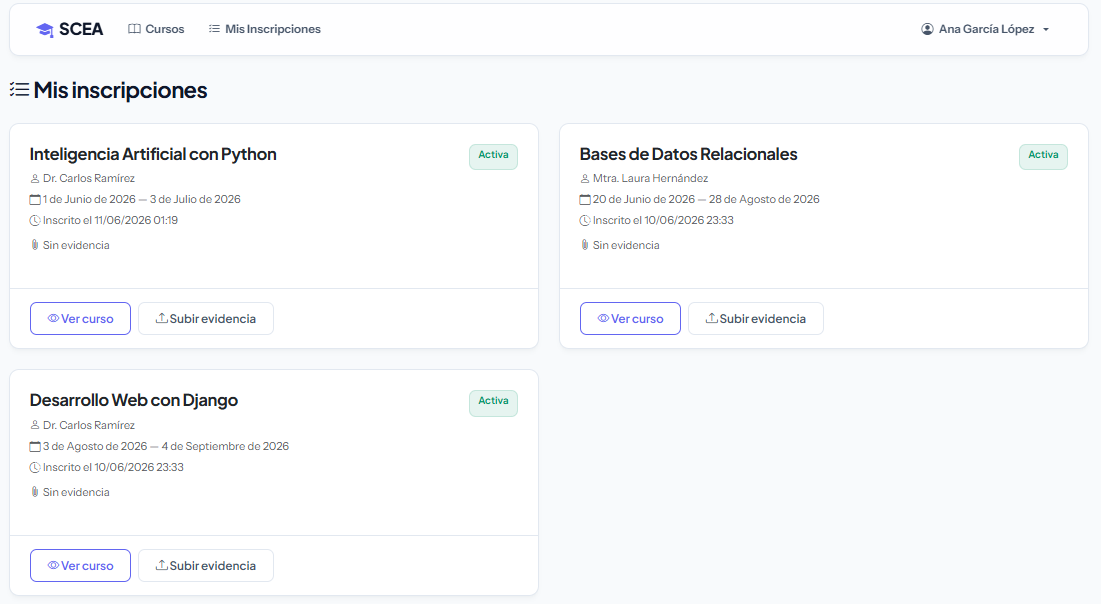
\includegraphics[width=\linewidth]{img/capturas_app/pagina_alumno.png}
			\caption{Vista Alumno}
		\end{subfigure}
		
		\caption{P\'agina de inicio con la barra de navegaci\'on diferenciada por rol (Mis Inscripciones para alumnos, Mis Cursos para instructores, Administrar para administradores).}
	\end{figure}
	\vspace{1cm}
	% ======================== 7. RF =======================================
	\section{Requerimientos funcionales}
	\begin{center}\small
		\begin{longtable}{|>{\bfseries}p{1.1cm}|p{3cm}|p{10.5cm}|}
			\hline
			\headrowcolor \headcell{ID} & \headcell{Nombre} & \headcell{Descripci\'on} \\ \hline \endhead
			RF01 & Registro de usuarios & El registro p\'ublico permite crear cuenta con nombre, apellidos, correo, usuario y contrase\~na. Por seguridad, el rol se asigna siempre como alumno (no hay selector de tipo en el formulario). \\
			 \hline
			\rowcolor{grisAlt}
			RF02 & Inicio y cierre de sesi\'on & Los usuarios registrados pueden autenticarse y cerrar sesi\'on. \\ \hline
			RF03 & Gesti\'on de alumnos & CRUD completo de alumnos (lista, crear, editar, eliminar) restringido a administradores, con validaciones de correo \'unico y nombre m\'inimo. \\ \hline
			\rowcolor{grisAlt}
			RF04 & Gesti\'on de instructores & CRUD completo restringido a administradores. Al crear, el formulario incluye usuario y contrase\~na; el sistema genera \texttt{User}, \texttt{PerfilUsuario} (instructor) e \texttt{Instructor} vinculados en una transacci\'on. \\ \hline
			RF05 & Gesti\'on de cursos & CRUD de cursos restringido a administradores; incluye carga de imagen, estado y cupo m\'aximo. \\ \hline
			\rowcolor{grisAlt}
			RF06 & Consulta de cursos & Los alumnos ven la lista de cursos disponibles con b\'usqueda y filtrado. \\ \hline
			RF07 & Inscripci\'on a cursos & Solo usuarios con rol alumno pueden inscribirse en l\'inea a un curso activo con cupo disponible. \\ \hline
			\rowcolor{grisAlt}
			RF08 & Validaci\'on de cupo & El sistema rechaza inscripciones cuando el curso alcanz\'o su cupo m\'aximo. \\ \hline
			RF09 & Evitar duplicados & Un mismo alumno no puede inscribirse dos veces al mismo curso (restricci\'on \texttt{unique\_together} a nivel de base de datos). \\ \hline
			\rowcolor{grisAlt}
			RF10 & Carga de evidencia & El alumno puede subir un archivo (PDF, imagen o Word) como comprobante de inscripci\'on. \\ \hline
			RF11 & Lista de inscritos & Administradores e instructores asignados consultan la lista de alumnos inscritos por curso. \\ \hline
			\rowcolor{grisAlt}
			RF12 & B\'usqueda y filtrado & B\'usqueda de cursos por nombre, nombre de instructor y estado. \\ \hline
			RF13 & Validaciones en formularios & Nombre m\'inimo 3 caracteres, correo \'unico, cupo mayor que cero, fecha de t\'ermino mayor o igual a la de inicio, tama\~no m\'aximo de archivos. \\ \hline
			\rowcolor{grisAlt}
			RF14 & Mensajes al usuario & Mensajes flash de \'exito, error o advertencia tras cada operaci\'on CRUD o inscripci\'on. \\ \hline
			RF15 & Protecci\'on de vistas & Inscripci\'on y evidencia: solo alumnos autenticados. CRUD web: solo administrador. Mis cursos: instructor o admin. Men\'u de navegaci\'on acorde al rol. \\ \hline
			\rowcolor{grisAlt}
			RF16 & API REST & Endpoints GET, POST, PUT, PATCH y DELETE para cursos, alumnos, inscripciones e instructores con permisos por rol. \\ \hline
		\end{longtable}
	\end{center}
	
	% ======================== 8. RNF ======================================
	\section{Requerimientos no funcionales}
	\begin{center}\small
		\begin{tabularx}{\linewidth}{|>{\bfseries}p{1.3cm}|p{3.2cm}|X|}
			\hline
			\headrowcolor \headcell{ID} & \headcell{Nombre} & \headcell{Descripci\'on} \\ \hline
			RNF01 & Usabilidad & La interfaz utiliza Bootstrap 5.3 y mantiene una navegaci\'on consistente e intuitiva que facilita el acceso a las funcionalidades principales del sistema. \\ \hline
			\rowcolor{grisAlt}
			RNF02 & Seguridad & Vistas sensibles protegidas con \texttt{@login\_required} y \texttt{UserPassesTestMixin} seg\'un el rol. \\ \hline
			RNF03 & Integridad de datos & Validaciones en formularios y serializers evitan registros duplicados e informaci\'on inv\'alida. \\ \hline
			\rowcolor{grisAlt}
			RNF04 & Mantenibilidad & C\'odigo organizado en apps (\texttt{usuarios}, \texttt{cursos}, \texttt{inscripciones}) con modelos, vistas, formularios, URLs y serializers separados. \\ \hline
			RNF05 & Escalabilidad & Arquitectura de apps independientes permite agregar m\'odulos (pagos, certificados, reportes) sin reestructurar el proyecto. \\ \hline
			\rowcolor{grisAlt}
			RNF06 & Rendimiento & El sistema mantiene tiempos de respuesta adecuados para entornos acad\'emicos y vol\'umenes peque\~nos o medianos de informaci\'on, peque\~nos o medianos con SQLite. \\ \hline
			RNF07 & Compatibilidad & Funciona en entorno local con Python 3.10+, Django~4.2, SQLite y cualquier sistema operativo que soporte Python. \\ \hline
			\rowcolor{grisAlt}
			RNF08 & Legibilidad del c\'odigo & Docstrings en clases y funciones clave; comentarios inline en validaciones cr\'iticas. \\ \hline
		\end{tabularx}
	\end{center}
	
	% ======================== 9. REGLAS DE NEGOCIO ========================
	\section{Reglas de negocio}
	Las siguientes reglas se aplican tanto en la capa de vistas como en la API REST:
	\begin{enumerate}[leftmargin=*]
		\item Un alumno no puede inscribirse dos veces al mismo curso. Restricci\'on \texttt{unique\_together('alumno','curso')} en el modelo \texttt{Inscripcion}.
		\item Un curso no puede aceptar m\'as alumnos que su cupo m\'aximo. Validado por el m\'etodo \texttt{tiene\_cupo()} en el modelo \texttt{Curso}.
		\item Un curso cancelado o cerrado no permite nuevas inscripciones. Validaci\'on de estado antes de crear inscripci\'on en vistas y serializers.
		\item La fecha de t\'ermino debe ser posterior o igual a la fecha de inicio. Implementado en \texttt{CursoForm.clean()} y \texttt{CursoSerializer.validate()}.
		\item Solo usuarios con rol alumno pueden inscribirse a cursos. La vista \texttt{inscribirse} verifica \texttt{perfil.es\_alumno()}.
		\item Solo administradores o el instructor asignado al curso pueden consultar la lista completa de alumnos inscritos.
		\item Solo administradores pueden crear, editar o eliminar cursos. Validado con \texttt{UserPassesTestMixin} y \texttt{perfil.es\_admin()}.
	\end{enumerate}
	
	% ======================== 10. MODELO DE DATOS =========================
	\section{Modelo de datos}
	El sistema usa SQLite y define cinco entidades principales mapeadas como modelos Django. A continuaci\'on se describe cada entidad con sus campos.
	
	\subsection{Entidad PerfilUsuario}
	\begin{center}\small
		\begin{tabularx}{\linewidth}{|p{3cm}|p{4cm}|X|}
			\hline
			\headrowcolor \headcell{Campo} & \headcell{Tipo} & \headcell{Descripci\'on} \\ \hline
			\texttt{usuario} & OneToOneField(User) & Relaci\'on 1:1 con el usuario de Django Auth. \\ \hline
			\rowcolor{grisAlt}
			\texttt{tipo} & CharField(choices) & Rol del usuario: alumno, instructor o admin. \\ \hline
		\end{tabularx}
	\end{center}
	
	\subsection{Entidad Alumno}
	\begin{center}\small
		\begin{tabularx}{\linewidth}{|p{3cm}|p{4cm}|X|}
			\hline
			\headrowcolor \headcell{Campo} & \headcell{Tipo} & \headcell{Descripci\'on} \\ \hline
			\texttt{usuario} & OneToOneField(User) & Relaci\'on opcional con la cuenta de Django Auth. \\ \hline
			\rowcolor{grisAlt}
			\texttt{nombre} & CharField(150) & Nombre completo del alumno. \\ \hline
			\texttt{correo} & EmailField(unique) & Correo electr\'onico \'unico. \\ \hline
			\rowcolor{grisAlt}
			\texttt{matricula} & CharField(20, unique) & Clave de identificaci\'on institucional. \\ \hline
			\texttt{telefono} & CharField(15, blank) & N\'umero de contacto opcional. \\ \hline
			\rowcolor{grisAlt}
			\texttt{foto} & ImageField(blank) & Fotograf\'ia del alumno (\texttt{media/miembros/}). \\ \hline
			\texttt{fecha\_registro} & DateField(auto) & Fecha en que se registr\'o en el sistema. \\ \hline
		\end{tabularx}
	\end{center}
	
	\subsection{Entidad Instructor}
	\begin{center}\small
		\begin{tabularx}{\linewidth}{|p{3cm}|p{4cm}|X|}
			\hline
			\headrowcolor \headcell{Campo} & \headcell{Tipo} & \headcell{Descripci\'on} \\ \hline
			\texttt{usuario} & OneToOneField(User) & Cuenta de acceso vinculada (creada por el admin al dar de alta). \\ \hline
			\rowcolor{grisAlt}
			\texttt{nombre} & CharField(150) & Nombre completo del instructor. \\ \hline
			\texttt{correo} & EmailField(unique) & Correo electr\'onico \'unico. \\ \hline
			\rowcolor{grisAlt}
			\texttt{especialidad} & CharField(200) & \'Area de conocimiento del instructor. \\ \hline
			\texttt{telefono} & CharField(15, blank) & N\'umero de contacto opcional. \\ \hline
		\end{tabularx}
	\end{center}
	
	\subsection{Entidad Curso}
	\begin{center}\small
		\begin{tabularx}{\linewidth}{|p{3cm}|p{4cm}|X|}
			\hline
			\headrowcolor \headcell{Campo} & \headcell{Tipo} & \headcell{Descripci\'on} \\ \hline
			\texttt{nombre} & CharField(200) & Nombre del curso o evento. \\ \hline
			\rowcolor{grisAlt}
			\texttt{descripcion} & TextField & Descripci\'on detallada del contenido. \\ \hline
			\texttt{fecha\_inicio} & DateField & Fecha de inicio del curso. \\ \hline
			\rowcolor{grisAlt}
			\texttt{fecha\_termino} & DateField & Fecha de conclusi\'on ($\geq$ \texttt{fecha\_inicio}). \\ \hline
			\texttt{cupo\_maximo} & PositiveIntegerField & N\'umero m\'aximo de alumnos permitidos. \\ \hline
			\rowcolor{grisAlt}
			\texttt{instructor} & ForeignKey(Instructor) & Instructor responsable (\texttt{NULL} si se elimina el instructor). \\ \hline
			\texttt{imagen} & ImageField(blank) & Imagen o portada del curso (\texttt{media/cursos/imagenes/}). \\ \hline
			\rowcolor{grisAlt}
			\texttt{estado} & CharField(choices) & Estado: activo, cerrado o cancelado. \\ \hline
			\texttt{fecha\_creacion} & DateTimeField(auto) & Marca de tiempo de creaci\'on autom\'atica. \\ \hline
		\end{tabularx}
	\end{center}
	
	\subsection{Entidad Inscripci\'on}
	\begin{center}\small
		\begin{tabularx}{\linewidth}{|p{3cm}|p{4cm}|X|}
			\hline
			\headrowcolor \headcell{Campo} & \headcell{Tipo} & \headcell{Descripci\'on} \\ \hline
			\texttt{alumno} & ForeignKey(Alumno) & Alumno que se inscribe. \\ \hline
			\rowcolor{grisAlt}
			\texttt{curso} & ForeignKey(Curso) & Curso al que se inscribe. \\ \hline
			\texttt{fecha\_inscripcion} & DateTimeField(auto) & Marca de tiempo autom\'atica al crear el registro. \\ \hline
			\rowcolor{grisAlt}
			\texttt{estado} & CharField(choices) & Estado de la inscripci\'on: activa, cancelada o completada. \\ \hline
			\texttt{evidencia} & FileField(blank) & Archivo comprobante subido por el alumno (\texttt{media/inscripciones/evidencias/}). \\ \hline
		\end{tabularx}
	\end{center}
	Restricci\'on de integridad: \texttt{unique\_together = ('alumno', 'curso')} impide inscripciones duplicadas a nivel de base de datos, dando soporte f\'isico al requerimiento RF09.
	
	% ======================== 11. ER ======================================
	\section{Diagrama entidad-relaci\'on}
	El siguiente diagrama muestra las entidades principales del sistema y sus relaciones, conforme al modelo de datos descrito en la secci\'on anterior.
	
	\figura[0.98]{img/ER_diagram.png}{Diagrama entidad-relaci\'on generado a partir de los modelos Django del sistema}
	
	Relaciones implementadas:
	\begin{itemize}[leftmargin=*]
		\item \texttt{User} (Django Auth) 1:1 \texttt{PerfilUsuario} -- cada usuario tiene exactamente un perfil con rol asignado.
		\item \texttt{User} 1:1 \texttt{Alumno} -- un usuario de tipo alumno se vincula con un perfil acad\'emico de Alumno.
		\item \texttt{User} 1:1 \texttt{Instructor} -- un usuario de tipo instructor se vincula con un perfil de Instructor.
		\item \texttt{Instructor} 1:N \texttt{Curso} -- un instructor puede impartir muchos cursos; un curso tiene como m\'aximo un instructor asignado.
		\item \texttt{Alumno} N:M \texttt{Curso} a trav\'es de \texttt{Inscripcion} -- un alumno puede inscribirse a varios cursos y un curso puede tener varios alumnos inscritos.
		\item \texttt{Inscripcion} contiene el archivo de evidencia, por lo que la relaci\'on con archivos se da a trav\'es de este modelo intermedio.
	\end{itemize}
	
	% ======================== 12. VISTAS ==================================
	\section{Descripci\'on de vistas principales}
	El sistema combina vistas basadas en funciones (FBV) para flujos sencillos y vistas basadas en clases (CBV) para los CRUD principales, cumpliendo as\'i con el requisito del uso de \texttt{ListView}, \texttt{DetailView}, \texttt{CreateView}, \texttt{UpdateView} y \texttt{DeleteView}.
	
	\begin{center}\small
		\begin{longtable}{|p{5.2cm}|p{2.4cm}|p{7.2cm}|}
			\hline
			\headrowcolor \headcell{URL / Vista} & \headcell{Tipo} & \headcell{Descripci\'on y restricciones} \\ \hline \endhead
			\texttt{/} (inicio) & FBV & P\'agina de inicio con hasta 6 cursos activos destacados. Accesible para todos. \\ \hline
			\rowcolor{grisAlt}
			\texttt{/cursos/} (\texttt{CursoListView}) & CBV ListView & Lista de cursos con b\'usqueda por nombre, instructor y estado. P\'ublica. \\ \hline
			\texttt{/cursos/<id>/} (\texttt{CursoDetailView}) & CBV DetailView & Detalle del curso y cupo disponible. Bot\'on \emph{Inscribirse} solo si es alumno y hay cupo. \\ \hline
			\rowcolor{grisAlt}
			\texttt{/cursos/mis-cursos/} & CBV ListView & \texttt{CursoInstructorListView}. Cursos que imparte el instructor autenticado. \\ \hline
			\texttt{/cursos/nuevo/} & CBV CreateView & Formulario de creaci\'on de curso. Solo administradores. \\ \hline
			\rowcolor{grisAlt}
			\texttt{/cursos/<id>/editar/} & CBV UpdateView & Edici\'on de curso existente. Solo administradores. \\ \hline
			\texttt{/cursos/<id>/eliminar/} & CBV DeleteView & Confirmaci\'on y eliminaci\'on de curso. Solo administradores. \\ \hline
			\rowcolor{grisAlt}
			\texttt{/usuarios/registro/} & FBV & Registro p\'ublico solo para alumnos. Crea \texttt{PerfilUsuario} tipo alumno y matr\'icula \texttt{AL\#\#\#\#}. \\ \hline
			\texttt{/usuarios/login/} & FBV & Formulario de inicio de sesi\'on. \\ \hline
			\rowcolor{grisAlt}
			\texttt{/usuarios/logout/} & FBV & Cierre de sesi\'on y redirecci\'on a login. \\ \hline
			\texttt{/usuarios/perfil/} & FBV & Vista del perfil del usuario autenticado. \\ \hline
			\rowcolor{grisAlt}
			\texttt{/usuarios/alumnos/} & CBV & \texttt{AlumnoListView} con b\'usqueda. CRUD completo solo admin. \\ \hline
			\texttt{/usuarios/instructores/} & CBV & \texttt{InstructorListView} con columna de usuario de acceso. Solo administradores. \\ \hline
			\rowcolor{grisAlt}
			\texttt{/usuarios/instructores/nuevo/} & CBV & \texttt{InstructorCreateView} con \texttt{InstructorCreateForm}: crea \texttt{User} + \texttt{PerfilUsuario} + \texttt{Instructor} en una transacci\'on. \\ \hline
			\texttt{/inscripciones/gestion/} & CBV & \texttt{InscripcionListView}. Lista, b\'usqueda y CRUD administrativo de inscripciones. \\ \hline
			\rowcolor{grisAlt}
			\texttt{/inscripciones/mis-inscripciones/} & FBV & Lista de cursos en los que el alumno est\'a inscrito. Requiere rol alumno. \\ \hline
			\texttt{/inscripciones/inscribirse/<id>/} & FBV & Procesa la inscripci\'on solo si \texttt{perfil.es\_alumno()}; valida cupo, estado y duplicados. \\ \hline
			\rowcolor{grisAlt}
			\texttt{/inscripciones/<id>/evidencia/} & FBV & Formulario para subir archivo de evidencia. Solo el alumno propietario. \\ \hline
			\texttt{/inscripciones/curso/<id>/inscritos/} & FBV & Lista de alumnos inscritos. Solo admin o instructor asignado. \\ \hline
			\rowcolor{grisAlt}
			\texttt{/admin/} & Django Admin & Panel nativo de administraci\'on con acceso a todos los modelos registrados. \\ \hline
		\end{longtable}
	\end{center}
	
	\subsection{Navegaci\'on principal (\texttt{templates/base.html})}
	\begin{center}\small
		\begin{tabularx}{\linewidth}{|p{5cm}|X|}
			\hline
			\headrowcolor \headcell{Elemento del men\'u} & \headcell{Visible para} \\ \hline
			Cursos & Todos los usuarios \\ \hline
			\rowcolor{grisAlt}
			Mis Inscripciones & Solo \texttt{perfil.tipo == 'alumno'} \\ \hline
			Mis Cursos & Solo \texttt{perfil.tipo == 'instructor'} \\ \hline
			\rowcolor{grisAlt}
			Administrar (dropdown) & Solo admin (\texttt{is\_staff} o \texttt{perfil.tipo == 'admin'}) \\ \hline
		\end{tabularx}
	\end{center}
	
	% ======================== 13. FORMULARIOS =============================
	\section{Descripci\'on de formularios y validaciones}
	
	\subsection{RegistroUsuarioForm (\texttt{usuarios/forms.py})}
	Extiende \texttt{UserCreationForm} de Django. Campos adicionales: \texttt{first\_name}, \texttt{last\_name} y \texttt{email}. Validaciones:
	\begin{itemize}[leftmargin=*]
		\item \texttt{clean\_first\_name}: rechaza nombres con menos de 3 caracteres.
		\item \texttt{clean\_email}: verifica que el correo no est\'e registrado previamente en la tabla \texttt{auth\_user}.
		\item \texttt{save}: crea el usuario, asigna \texttt{PerfilUsuario} con tipo alumno y crea el registro \texttt{Alumno} vinculado con matr\'icula autom\'atica (\texttt{AL\#\#\#\#}).
	\end{itemize}
	
	\subsection{CursoForm (\texttt{cursos/forms.py})}
	\texttt{ModelForm} basado en \texttt{Curso} con widgets Bootstrap. Validaciones:
	\begin{itemize}[leftmargin=*]
		\item \texttt{clean\_nombre}: longitud m\'inima de 3 caracteres.
		\item \texttt{clean\_cupo\_maximo}: debe ser mayor que cero.
		\item \texttt{clean\_imagen}: tama\~no m\'aximo 5~MB; solo se aceptan JPEG, PNG, GIF o WebP.
		\item \texttt{clean}: validaci\'on cruzada \texttt{fecha\_termino} $\geq$ \texttt{fecha\_inicio}.
	\end{itemize}
	
	\subsection{AlumnoForm (\texttt{usuarios/forms.py})}
	\texttt{ModelForm} basado en \texttt{Alumno}. Validaciones:
	\begin{itemize}[leftmargin=*]
		\item \texttt{clean\_nombre}: m\'inimo 3 caracteres.
		\item \texttt{clean\_correo}: unicidad excluyendo el propio registro al editar.
		\item \texttt{clean\_foto}: tama\~no m\'aximo 2~MB y tipos de imagen v\'alidos.
	\end{itemize}
	
	\subsection{InstructorCreateForm (\texttt{usuarios/forms.py})}
	Extiende \texttt{InstructorForm} para el alta por administrador. Campos adicionales: \texttt{username}, \texttt{password1}, \texttt{password2}. Validaciones:
	\begin{itemize}[leftmargin=*]
		\item \texttt{clean\_username}: unicidad en \texttt{auth\_user}.
		\item \texttt{clean\_correo}: unicidad en \texttt{Instructor} y en \texttt{User.email}.
		\item \texttt{clean\_password2}: las contrase\~nas deben coincidir.
		\item \texttt{save} (transacci\'on at\'omica): crea \texttt{User}, \texttt{PerfilUsuario} (instructor), vincula \texttt{Instructor.usuario} y guarda la ficha.
	\end{itemize}
	
	\subsection{InstructorForm (\texttt{usuarios/forms.py})}
	\texttt{ModelForm} para edici\'on de \texttt{Instructor}. Valida nombre, correo y unicidad en \texttt{User.email} si hay cuenta vinculada. El m\'etodo \texttt{save} sincroniza \texttt{correo}, \texttt{first\_name} y \texttt{last\_name} del \texttt{User} vinculado.
	
	\subsection{InscripcionForm (\texttt{inscripciones/forms.py})}
	\texttt{ModelForm} para gesti\'on administrativa de inscripciones. Campos: \texttt{alumno}, \texttt{curso}, \texttt{estado} y \texttt{evidencia}. Validaciones:
	\begin{itemize}[leftmargin=*]
		\item \texttt{clean}: evita duplicados alumno-curso; en creaci\'on valida el estado del curso y el cupo disponible.
		\item \texttt{clean\_evidencia}: tama\~no m\'aximo 10~MB; extensiones \texttt{.pdf}, \texttt{.png}, \texttt{.jpg}, \texttt{.jpeg}, \texttt{.doc}, \texttt{.docx}.
	\end{itemize}
	
	\subsection{EvidenciaForm (\texttt{inscripciones/forms.py})}
	\texttt{ModelForm} que actualiza \'unicamente el campo \texttt{evidencia} de \texttt{Inscripcion} para el alumno propietario. Aplica las mismas reglas de archivo que \texttt{InscripcionForm} en \texttt{clean\_evidencia}.
	
	\subsection{BusquedaCursoForm (\texttt{cursos/forms.py})}
	Formulario de b\'usqueda no vinculado a modelo. Campos: \texttt{q} (texto libre), \texttt{estado} (choice) e \texttt{instructor} (texto libre). Todos opcionales.
	
	\figura[0.90]{img/capturas_app/editar_curso_admin.png}{Formulario de edici\'on de curso con campos y validaciones (CursoForm)}
	
	% ======================== 14. API REST ================================
	\section{Descripci\'on de la API REST}
	La API REST se implementa con Django REST Framework usando \texttt{ModelViewSet} y un router que genera autom\'aticamente las URLs est\'andar. Es navegable desde el navegador en \url{http://127.0.0.1:8000/api/}.
	
	\subsection{Endpoints disponibles}
	\begin{center}\small
		\begin{longtable}{|p{4.3cm}|p{3.3cm}|p{7.2cm}|}
			\hline
			\headrowcolor \headcell{Endpoint} & \headcell{M\'etodos} & \headcell{Descripci\'on y permisos} \\ \hline \endhead
			\texttt{/api/cursos/} & GET, POST & GET p\'ublico; POST solo administrador. \\ \hline
			\rowcolor{grisAlt}
			\texttt{/api/cursos/<id>/} & GET, PUT, PATCH, DELETE & GET p\'ublico; PUT, PATCH y DELETE solo administrador. \\ \hline
			\texttt{/api/cursos/<id>/inscritos/} & GET & Lista inscripciones del curso. Solo admin o instructor asignado. \\ \hline
			\rowcolor{grisAlt}
			\texttt{/api/alumnos/} & GET, POST & GET: admin o instructor; POST: solo admin. \\ \hline
			\texttt{/api/alumnos/<id>/} & GET, PUT, PATCH, DELETE & GET/PUT/PATCH: admin, instructor o el propio alumno. DELETE: solo admin. \\ \hline
			\rowcolor{grisAlt}
			\texttt{/api/inscripciones/} & GET, POST & GET filtrado por rol; POST: alumno solo para s\'i mismo, admin puede crear cualquiera. \\ \hline
			\texttt{/api/inscripciones/<id>/} & GET, PUT, PATCH, DELETE & GET: due\~no, instructor del curso o admin; PUT/PATCH: due\~no o admin; DELETE: solo admin. \\ \hline
			\rowcolor{grisAlt}
			\texttt{/api/instructores/} & GET, POST & GET: cualquier usuario autenticado; POST: solo admin. \\ \hline
			\texttt{/api/instructores/<id>/} & GET, PUT, PATCH, DELETE & GET: autenticado; PUT/PATCH: admin o el propio instructor; DELETE: solo admin. \\ \hline
			\rowcolor{grisAlt}
			\texttt{/api-auth/} & GET, POST & Login/logout de la API navegable de DRF. \\ \hline
		\end{longtable}
	\end{center}
	
	\subsection{Serializers}
	\begin{itemize}[leftmargin=*]
		\item \textbf{CursoSerializer:} incluye campos calculados \texttt{instructor\_nombre} y \texttt{cupo\_disponible} (read\_only). Valida fechas y cupo.
		\item \textbf{AlumnoSerializer:} expone \texttt{id}, \texttt{nombre}, \texttt{correo}, \texttt{matricula}, \texttt{telefono} y \texttt{fecha\_registro}.
		\item \textbf{InscripcionSerializer:} incluye \texttt{alumno\_nombre} y \texttt{curso\_nombre} como campos de solo lectura derivados.
		\item \textbf{InstructorSerializer:} expone \texttt{id}, \texttt{nombre}, \texttt{correo}, \texttt{especialidad} y \texttt{telefono}.
	\end{itemize}
	
	\subsection{Permisos}
	La API usa clases de permiso personalizadas adem\'as de las nativas de DRF:
	\begin{itemize}[leftmargin=*]
		\item \textbf{CursoViewSet:} \texttt{AllowAny} en lectura; \texttt{IsAdminUser} en create, update y destroy; \texttt{IsAdminOrCourseInstructor} en la acci\'on \texttt{inscritos}.
		\item \textbf{AlumnoViewSet:} \texttt{IsAdminUser} en create y destroy; \texttt{IsAdminOrInstructorOrSelf} en list, retrieve, update y partial\_update.
		\item \textbf{InscripcionViewSet:} \texttt{get\_queryset()} filtra por rol; \texttt{IsInscripcionOwnerOrInstructorOrAdmin} en operaciones sobre objetos; \texttt{IsAdminUser} en destroy.
		\item \textbf{InstructorViewSet:} \texttt{IsAdminUser} en create y destroy; \texttt{IsAdminOrSelfOrReadOnlyAuthenticated} en el resto.
	\end{itemize}
	
	\figura[0.95]{img/capturas_app/api_curso.png}{API REST navegable de DRF mostrando la respuesta JSON del endpoint \texttt{/api/cursos/}}
	
	% ======================== 15. CAPTURAS ================================
	\section{Capturas de pantalla}
	Se presentan las pantallas principales del sistema en funcionamiento. Las capturas cubren los flujos m\'as importantes: acceso p\'ublico, autenticaci\'on, gesti\'on de cursos y de inscripciones, y la API REST navegable.
	
	\figura[0.92]{img/capturas_app/home_alumno.png}{P\'agina de inicio (\texttt{/}) con los cursos activos destacados}
	
	\figura[0.88]{img/capturas_app/registro.png}{Formulario de registro p\'ublico de alumno (\texttt{/usuarios/registro/})}
	
	\figura[0.88]{img/capturas_app/logIn.png}{Formulario de inicio de sesi\'on (\texttt{/usuarios/login/})}
	
	\figura[0.92]{img/capturas_app/lista_curso_admin_filtro.png}{Cat\'alogo de cursos (\texttt{/cursos/}) con b\'usqueda y filtros aplicados}
	
	\figura[0.92]{img/capturas_app/vista_curso_alumno.png}{Detalle de un curso con bot\'on Inscribirse (vista de alumno)}
	
	\figura[0.92]{img/capturas_app/lista_curso_admin.png}{Lista de cursos con panel de administraci\'on (vista de administrador)}
	
	\figura[0.88]{img/capturas_app/inscripciones_alumno.png}{Vista Mis Inscripciones del alumno (\texttt{/inscripciones/mis-inscripciones/})}
	
	\figura[0.88]{img/capturas_app/mis_cursos_alumno.png}{Vista de cursos disponibles para inscripci\'on del alumno}
	
	\figura[0.92]{img/capturas_app/mis_cursos_instructor.png}{Vista Mis Cursos del instructor (\texttt{/cursos/mis-cursos/})}
	
	\figura[0.90]{img/capturas_app/alumnos_inscritos_instructor.png}{Lista de alumnos inscritos por curso (vista de admin/instructor)}
	
	\figura[0.90]{img/capturas_app/gestion_inscripciones_admin.png}{Gesti\'on administrativa de inscripciones (\texttt{/inscripciones/gestion/})}
	
	\figura[0.88]{img/capturas_app/registrar_instructor_admin.png}{Alta de instructor con usuario y contrase\~na (InstructorCreateForm)}
	
	\figura[0.88]{img/capturas_app/crear_curso_admin.png}{Formulario de creaci\'on de curso (CursoForm)}
	
	\figura[0.92]{img/capturas_app/Api_root.png}{API REST navegable de DRF (p\'agina ra\'iz \texttt{/api/})}
	
	% ======================== 16. PRUEBAS =================================
	\section{Pruebas realizadas}
	Se dise\~n\'o un plan de pruebas estructurado que combina pruebas manuales, pruebas unitarias, pruebas de integraci\'on, pruebas de seguridad por rol y pruebas de interfaz automatizadas con Selenium WebDriver. La cobertura final fue de \textbf{20 casos de prueba manuales} y \textbf{55 pruebas automatizadas}, todas con resultado exitoso.
	
	\subsection{Resumen de cobertura}
	\begin{center}\small
		\begin{tabularx}{\linewidth}{|X|c|p{4.5cm}|}
			\hline
			\headrowcolor \headcell{Tipo de prueba} & \headcell{Cantidad} & \headcell{Casos asociados} \\ \hline
			Pruebas de registro o alta de informaci\'on & 4 & CP-01, CP-02, CP-03, CP-04 \\ \hline
			\rowcolor{grisAlt}
			Pruebas de consulta o listado & 2 & CP-06, CP-08 \\ \hline
			Pruebas de edici\'on o eliminaci\'on & 4 & CP-09, CP-10, CP-11, CP-12 \\ \hline
			\rowcolor{grisAlt}
			Pruebas de validaci\'on de datos & 3 & CP-13, CP-14, CP-15 \\ \hline
			Pruebas de reglas de negocio & 2 & CP-16, CP-17 \\ \hline
			\rowcolor{grisAlt}
			Pruebas de navegaci\'on o interfaz & 2 & CP-18, CP-19 \\ \hline
			Pruebas libres del equipo & 3 & CP-05, CP-07, CP-20 \\ \hline
			\rowcolor{grisAlt}
			\textbf{Total casos manuales} & \textbf{20} & --- \\ \hline
			Pruebas automatizadas (pytest + Selenium) & 55 & Suite completa \\ \hline
		\end{tabularx}
	\end{center}
	
	\subsection{Pruebas de l\'ogica y validaciones}
	\begin{center}\small
		\begin{tabularx}{\linewidth}{|p{4.2cm}|X|c|}
			\hline
			\headrowcolor \headcell{Caso} & \headcell{Resultado esperado} & \headcell{Estado} \\ \hline
			L\'ogica del modelo Curso & \texttt{cupo\_disponible()} resta los alumnos activos del cupo m\'aximo; \texttt{tiene\_cupo()} devuelve disponibilidad. & Exitoso \\ \hline
			\rowcolor{grisAlt}
			Restricci\'on de inscripci\'on \'unica & \texttt{unique\_together('alumno','curso')} rechaza inscripciones duplicadas. & Exitoso \\ \hline
			Validaci\'on del cupo del curso & \texttt{CursoForm} rechaza cupos menores o iguales a cero. & Exitoso \\ \hline
			\rowcolor{grisAlt}
			Validaci\'on de fechas del curso & \texttt{CursoForm} rechaza fecha de t\'ermino anterior a inicio. & Exitoso \\ \hline
			Validaci\'on de registro de usuarios & \texttt{RegistroUsuarioForm} rechaza correos duplicados. & Exitoso \\ \hline
			\rowcolor{grisAlt}
			Validaci\'on de archivo de evidencia & \texttt{EvidenciaForm} rechaza archivos $>10$~MB o extensiones prohibidas. & Exitoso \\ \hline
			Validaciones de Alumno e Instructor & Correos duplicados y nombres $<3$ caracteres son rechazados. & Exitoso \\ \hline
		\end{tabularx}
	\end{center}
	
	\subsection{Pruebas de seguridad y control de acceso}
	\begin{center}\small
		\begin{tabularx}{\linewidth}{|p{4.2cm}|X|c|}
			\hline
			\headrowcolor \headcell{Caso} & \headcell{Resultado esperado} & \headcell{Estado} \\ \hline
			Protecci\'on de vistas an\'onimas & Usuarios an\'onimos redirigidos al login en \texttt{inscribirse}, \texttt{mis\_inscripciones} y \texttt{subir\_evidencia}. & Exitoso \\ \hline
			\rowcolor{grisAlt}
			Permisos CRUD de cursos (web) & Solo admin puede crear, editar o eliminar cursos; otros reciben HTTP 403. & Exitoso \\ \hline
			Acceso a lista de inscritos & Alumnos no acceden; solo admin o instructor asignado. & Exitoso \\ \hline
			\rowcolor{grisAlt}
			Protecci\'on de evidencias & Un alumno no puede modificar la evidencia de inscripciones ajenas. & Exitoso \\ \hline
			Permisos CRUD Alumnos / Instructores & Solo admin; otros reciben HTTP 403. & Exitoso \\ \hline
			\rowcolor{grisAlt}
			Permisos CRUD Inscripciones (web) & \texttt{/inscripciones/gestion/} solo accesible para administradores. & Exitoso \\ \hline
			Vista Mis cursos & Solo accesible para instructores autenticados. & Exitoso \\ \hline
			\rowcolor{grisAlt}
			Inscripci\'on en l\'inea & Admin e instructores no ven el bot\'on; la URL rechaza roles distintos de alumno. & Exitoso \\ \hline
			\rowcolor{grisAlt}
			Men\'u Mis Inscripciones & Solo visible para alumnos; admin e instructores no ven esta pesta\~na en la barra de navegaci\'on. & Exitoso \\ \hline
			Alta de instructor con cuenta & \texttt{InstructorCreateForm} crea \texttt{User}, \texttt{PerfilUsuario} e \texttt{Instructor} en una transacci\'on at\'omica. & Exitoso \\ \hline
			\rowcolor{grisAlt}
			Permisos API REST & Cada ViewSet aplica los permisos descritos en 14.3. & Exitoso \\ \hline
			Cierre de sesi\'on & Logout destruye la sesi\'on activa y bloquea acceso a vistas privadas. & Exitoso \\ \hline
		\end{tabularx}
	\end{center}
	
	\subsection{Pruebas de reglas de negocio de inscripci\'on}
	\begin{center}\small
		\begin{tabularx}{\linewidth}{|p{4.2cm}|X|c|}
			\hline
			\headrowcolor \headcell{Caso} & \headcell{Resultado esperado} & \headcell{Estado} \\ \hline
			Inscripci\'on en curso cancelado & El sistema devuelve error y rechaza la inscripci\'on. & Exitoso \\ \hline
			\rowcolor{grisAlt}
			Inscripci\'on en curso cerrado & Rechazo con mensaje de alerta. & Exitoso \\ \hline
			Inscripci\'on en curso lleno & Alerta de cupo lleno y no se guarda el registro. & Exitoso \\ \hline
			\rowcolor{grisAlt}
			Carga de evidencia exitosa & Archivo v\'alido guardado y confirmaci\'on visual. & Exitoso \\ \hline
			B\'usqueda y filtrado de cursos & Respuesta HTML contiene solo cursos coincidentes. & Exitoso \\ \hline
		\end{tabularx}
	\end{center}
	
	\subsection{Pruebas de la API REST e interfaz de usuario}
	Para verificar el comportamiento de la API REST se ejecut\'o una colecci\'on de Postman ubicada en \texttt{Entregables/Scea - Sistema de gesti\'on de cursos (pruebas api completas).postman\_collection.json}. Todas las operaciones obtuvieron c\'odigos 200/201/204 en operaciones permitidas y 401/403 en operaciones restringidas seg\'un el rol.
	
	Las pruebas de interfaz se automatizaron con Selenium WebDriver sobre Google Chrome:
	\begin{center}\small
		\begin{tabularx}{\linewidth}{|p{4.8cm}|X|c|}
			\hline
			\headrowcolor \headcell{Caso} & \headcell{Resultado} & \headcell{Estado} \\ \hline
			\texttt{test\_registro\_e\_inicio\_sesion} & Registro de alumno, redirecci\'on al login, autenticaci\'on y entrada al sistema. & Exitoso \\ \hline
			\rowcolor{grisAlt}
			\texttt{test\_inscripcion\_visual} & Navegaci\'on al cat\'alogo, clic en Inscribirse y verificaci\'on de la alerta de \'exito. & Exitoso \\ \hline
			\texttt{test\_subida\_archivo} & Carga de evidencia desde Mis Inscripciones con confirmaci\'on visual. & Exitoso \\ \hline
			\rowcolor{grisAlt}
			\texttt{test\_cierre\_sesion} & Cierre de sesi\'on y bloqueo de acceso a vistas privadas. & Exitoso \\ \hline
			\texttt{test\_filtrado\_catalogo\_cursos} & B\'usqueda y filtrado visual de cursos en el cat\'alogo. & Exitoso \\ \hline
		\end{tabularx}
	\end{center}

	\subsubsection{Evidencias de pruebas manuales}
	Durante la ejecuci\'on manual del plan de pruebas se capturaron las siguientes pantallas como evidencia del correcto funcionamiento de los flujos principales:

	\figura[0.85]{img/pruebas_test/manuales/registro_alumno.png}{CP-01: Registro p\'ublico de alumno -- confirmaci\'on de cuenta creada con rol asignado autom\'aticamente}

	\figura[0.85]{img/pruebas_test/manuales/curso_nuevo.png}{CP-02: Alta de curso por administrador -- mensaje de \'exito tras guardar}

	\figura[0.88]{img/pruebas_test/manuales/curso_nuevo2.png}{CP-02: Tarjeta del nuevo curso disponible en el cat\'alogo}

	\figura[0.85]{img/pruebas_test/manuales/inscribirse_curso.png}{CP-20: Flujo de inscripci\'on interactiva -- alerta de confirmaci\'on visible para el alumno}

	\figura[0.85]{img/pruebas_test/manuales/consulta_api_cusos.png}{CP-07: Consulta p\'ublica de cursos v\'ia API REST -- respuesta JSON con c\'odigo 200 OK}

	\subsection{Defectos detectados y corregidos}
	Durante la ejecuci\'on del plan de pruebas se identificaron y resolvieron los siguientes defectos:
	\begin{center}\small
		\begin{tabularx}{\linewidth}{|c|X|c|X|}
			\hline
			\headrowcolor \headcell{ID} & \headcell{Defecto} & \headcell{Severidad} & \headcell{Resoluci\'on} \\ \hline
			DEF-01 & \texttt{CursoUpdateView} permit\'ia guardar el campo nombre vac\'io o con solo espacios. & Menor & Se a\~nadi\'o validaci\'on en \texttt{CursoForm.clean\_nombre()} para exigir m\'inimo 3 caracteres reales. \\ \hline
			\rowcolor{grisAlt}
			DEF-02 & \texttt{cupo\_disponible()} filtraba por \texttt{estado='activo'} en lugar de \texttt{'activa'}, por lo que las inscripciones activas no se restaban del cupo. & Alta & Se corrigi\'o la consulta en \texttt{cursos/models.py} y se ajustaron las pruebas unitarias en \texttt{tests/test\_cursos.py}. \\ \hline
		\end{tabularx}
	\end{center}
	
	\figura[0.95]{img/pruebas_test/pytest_selenium/evidencia_pruebas_completas.png}{Ejecuci\'on de la suite completa: 55 pruebas automatizadas con resultado PASSED}
	
	\figura[0.90]{img/pruebas_test/pytest_selenium/test_cursos_ind.png}{Resultados detallados de las pruebas del m\'odulo de cursos}
	
	\figura[0.90]{img/pruebas_test/pytest_selenium/test_inscripciones_ind.png}{Resultados detallados de las pruebas del m\'odulo de inscripciones}
	
	\figura[0.90]{img/pruebas_test/pytest_selenium/test_selenium_ind.png}{Resultados de las pruebas de interfaz automatizadas con Selenium WebDriver}
	
	\figura[0.92]{img/pruebas_test/bugs/bug_nombre_curso.png}{DEF-01: Bug detectado -- campo nombre vac\'io aceptado en \texttt{CursoUpdateView} antes de la correcci\'on}
	
	\figura[0.92]{img/pruebas_test/bugs/bug_disponibilidad_curso.png}{DEF-02: Bug detectado -- \texttt{cupo\_disponible()} filtraba por estado incorrecto antes de la correcci\'on}
	
	% ======================== 17. CONCLUSIONES ============================
	\section{Conclusiones}
	El desarrollo del Sistema Web de Gesti\'on de Cursos, Eventos e Inscripciones Acad\'emicas permiti\'o aplicar de manera pr\'actica los conocimientos adquiridos durante el curso, integrando en un mismo proyecto conceptos relacionados con desarrollo web, bases de datos, validaci\'on de informaci\'on, control de acceso y consumo de servicios mediante API REST.
	
	A lo largo de la implementaci\'on se comprob\'o la importancia de establecer reglas de negocio claras y mecanismos de validaci\'on que permitan mantener la consistencia de los datos. Funcionalidades como el control de cupo, la prevenci\'on de inscripciones duplicadas, la gesti\'on de usuarios por roles y la carga de evidencias digitales contribuyen a que el sistema responda adecuadamente a las necesidades planteadas desde el inicio del proyecto.
	
	La arquitectura basada en aplicaciones independientes (\texttt{usuarios}, \texttt{cursos} e \texttt{inscripciones}) favorece la organizaci\'on del c\'odigo y facilita futuras tareas de mantenimiento y ampliaci\'on. Asimismo, el uso de Django y Django REST Framework permiti\'o implementar una soluci\'on robusta que combina una interfaz web funcional con servicios REST capaces de exponer la informaci\'on de manera estructurada y segura.
	
	Las pruebas manuales y automatizadas realizadas durante el desarrollo permitieron verificar el correcto funcionamiento de los principales procesos del sistema, aportando confianza sobre la estabilidad de la aplicaci\'on y ayudando a identificar oportunamente los errores encontrados durante la fase de implementaci\'on.
	
	M\'as all\'a del cumplimiento de los requerimientos acad\'emicos, este proyecto represent\'o una experiencia pr\'actica para comprender c\'omo distintas tecnolog\'ias pueden integrarse para resolver una problem\'atica real. El resultado es una aplicaci\'on funcional que contribuye a mejorar la organizaci\'on y administraci\'on de cursos y eventos acad\'emicos dentro de una instituci\'on educativa.
	
	Como trabajo futuro, se considera la posibilidad de incorporar funcionalidades adicionales como el despliegue en un entorno de producci\'on con PostgreSQL, el env\'io autom\'atico de notificaciones por correo electr\'onico, la generaci\'on de constancias digitales y la inclusi\'on de m\'odulos de reportes y estad\'isticas que ampl\'ien las capacidades actuales del sistema.
	% ======================== 18. REFERENCIAS =============================
	\section{Referencias}
	\begin{itemize}[leftmargin=*]
		\item Django Software Foundation. (2024). \emph{Django documentation, version 4.2}. \url{https://docs.djangoproject.com/en/4.2/}
		\item Django REST Framework. (2024). \emph{Django REST Framework documentation}. \url{https://www.django-rest-framework.org/}
		\item Bootstrap. (2024). \emph{Bootstrap 5.3 Documentation}. \url{https://getbootstrap.com/docs/5.3/}
		\item Python Software Foundation. (2024). \emph{Python 3 Documentation}. \url{https://docs.python.org/3/}
		\item Pillow Contributors. (2024). \emph{Pillow (PIL Fork) documentation}. \url{https://pillow.readthedocs.io/}
		\item Selenium Project. (2024). \emph{Selenium WebDriver documentation}. \url{https://www.selenium.dev/documentation/}
		\item pytest-django. (2024). \emph{pytest-django documentation}. \url{https://pytest-django.readthedocs.io/}
	\end{itemize}
	
\end{document}
